\documentclass[10pt]{beamer}
\usepackage{newcent}
\usepackage[utf8]{inputenc}
%\usepackage[czech]{babel}
%\usepackage[T1]{fontenc}
\usepackage{hyperref}
\usepackage{xcolor}
\usepackage{fancyvrb}
\usepackage{graphicx}
\usepackage{listings}
\usepackage[font=footnotesize, labelformat=empty]{caption}
\usetheme{FIT}

%%%%%%%%%%%%%%%%%%%%%%%%%%%%%%%%%%%%%%%%%%%%%%%%%%%%%%%%%%%%%%%%%%
\title[Data Structures – Stack]{Data Structures – Stack}

\author[]{Maksim Kalutski}

\institute[]{Brno University of Technology, Faculty of Information Technology\\
Bo\v{z}et\v{e}chova 1/2. 612 66 Brno - Kr\'alovo Pole\\
xkalut00@stud.fit.vutbr.cz}

%\institute[]{Fakulta informačních technologií
%Vysokého učení technického v Brně\\
%Bo\v{z}et\v{e}chova 1/2. 612 66 Brno - Kr\'alovo Pole\\
%login@fit.vutbr.cz}

% České logo - Czech logo
% beamerouterthemeFIT.sty řádek 9: fitlogo1_cz

\date{\today}
%\date{} % bez data / without date

%%%%%%%%%%%%%%%%%%%%%%%%%%%%%%%%%%%%%%%%%%%%%%%%%%%%%%%%%%%%%%%%%%

\begin{document}

\frame[plain]{\titlepage}

\begin{frame}\frametitle{What is a Stack?}
    \begin{itemize}
		\item A linear data structure.
		\item Follows LIFO (Last In, First Out) principle.
		\item Elements are added and removed from the top only.
	\end{itemize}
\end{frame}

\begin{frame}\frametitle{Operations on a Stack}
    \begin{enumerate}
        \item \textbf{Push()}
        \begin{itemize}
            \item \textbf{Complexity:} O(1)
        \end{itemize}
        \item \textbf{Pop()}
                \begin{itemize}
            \item \textbf{Complexity:} O(1)
        \end{itemize}
        \item \textbf{Top()}
                \begin{itemize}
            \item \textbf{Complexity:} O(1)
        \end{itemize}
        \item \textbf{IsEmpty()}
                \begin{itemize}
            \item \textbf{Complexity:} O(1)
        \end{itemize}
    \end{enumerate}
\end{frame}

\begin{frame}\frametitle{Operations on a Stack – Push}
    \textbf{Push:} Adds an element to the top of the stack.
    \begin{figure}[h]
        \centering
        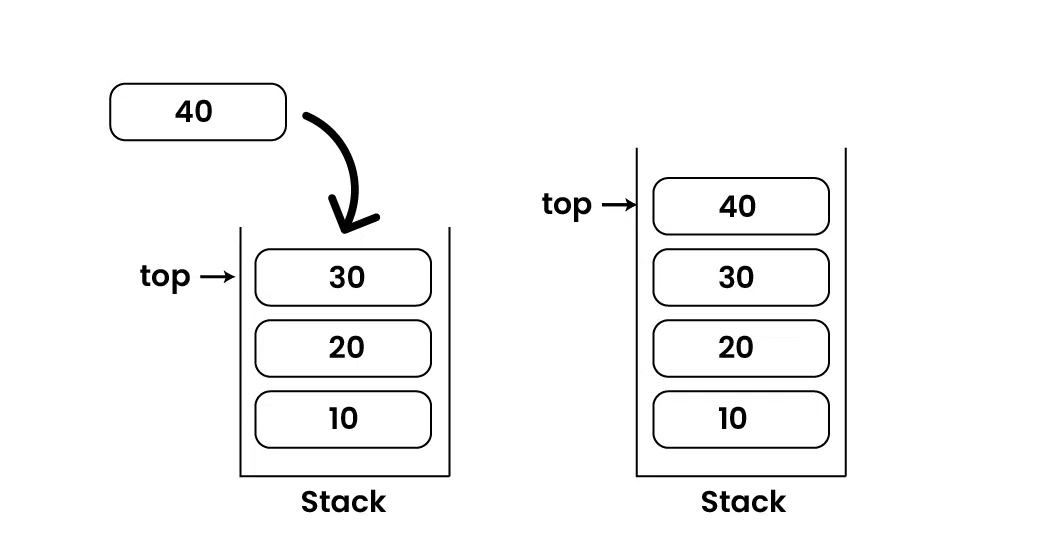
\includegraphics[width=1\textwidth]{img/push.png}
        \caption{Push operation on a stack. Source: \href{https://www.geeksforgeeks.org/introduction-to-stack-data-structure-and-algorithm-tutorials/}{geeksforgeeks}}
    \end{figure}
\end{frame}

\begin{frame}\frametitle{Operations on a Stack – Pop}
    \textbf{Pop:} Removes the top element from the stack.
        \begin{figure}[h]
        \centering
        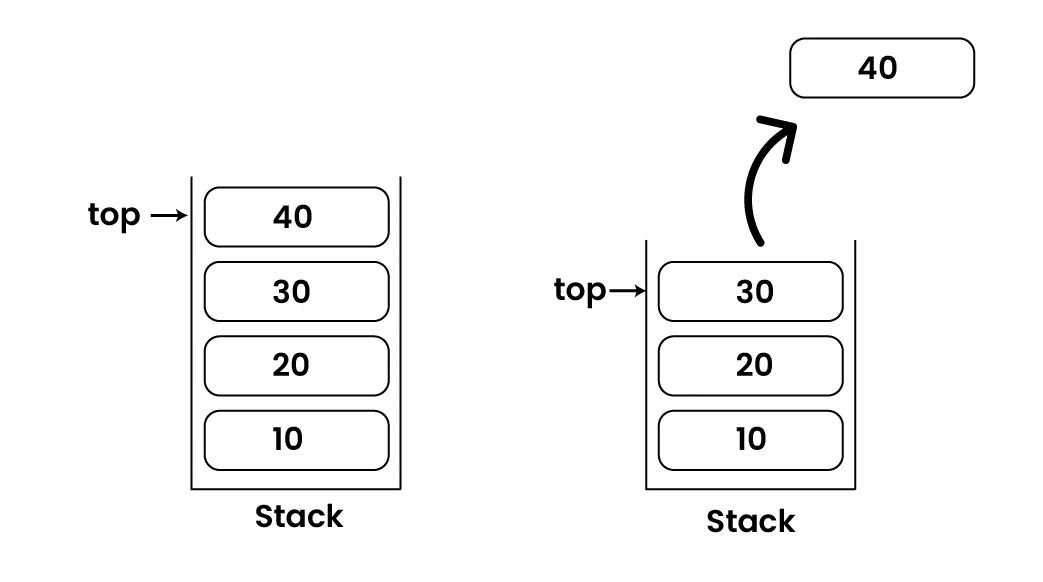
\includegraphics[width=1\textwidth]{img/pop.png}
        \caption{Pop operation on a stack. Source: \href{https://www.geeksforgeeks.org/introduction-to-stack-data-structure-and-algorithm-tutorials/}{geeksforgeeks}}
    \end{figure}
\end{frame}

\begin{frame}\frametitle{Operations on a Stack – Top}
    \textbf{Top:} Returns the value of the top element without removing it.
        \begin{figure}[h]
        \centering
        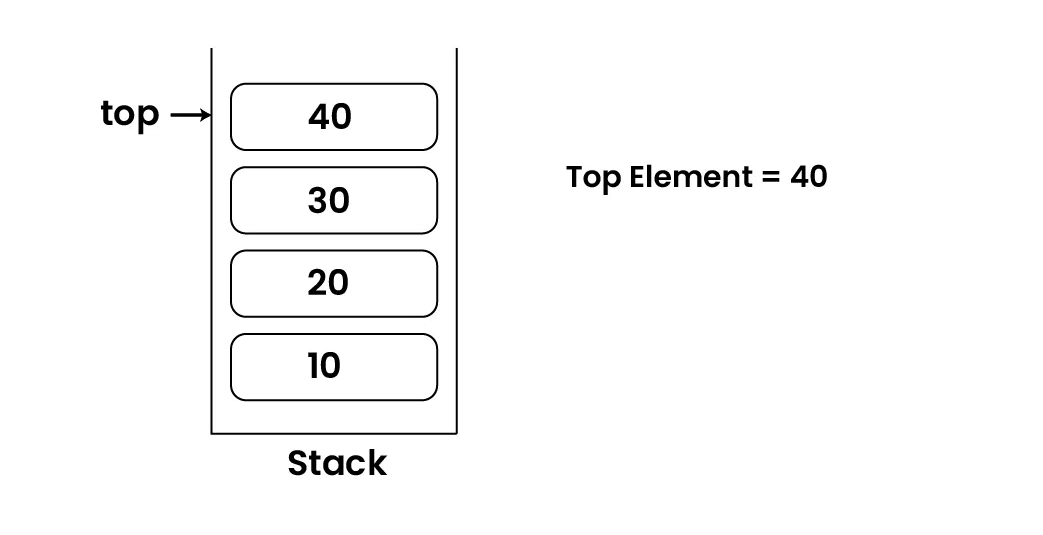
\includegraphics[width=1\textwidth]{img/top.png}
        \caption{Top operation on a stack. Source: \href{https://www.geeksforgeeks.org/introduction-to-stack-data-structure-and-algorithm-tutorials/}{geeksforgeeks}}
    \end{figure}
\end{frame}

\begin{frame}\frametitle{Operations on a Stack – IsEmpty}
    \textbf{IsEmpty:} Checks whether the stack is empty.
        \begin{figure}[h]
        \centering
        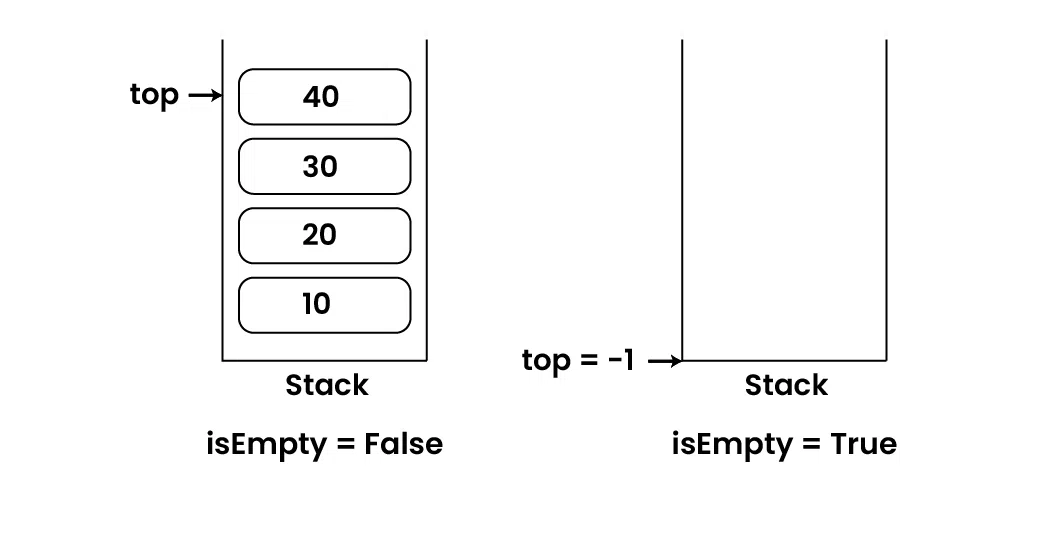
\includegraphics[width=1\textwidth]{img/isEmpty.png}
        \caption{IsEmpty operation on a stack. Source: \href{https://www.geeksforgeeks.org/introduction-to-stack-data-structure-and-algorithm-tutorials/}{geeksforgeeks}}
    \end{figure}
\end{frame}

\begin{frame}\frametitle{Implementation of Stack}
    \begin{itemize}
        \item Can be implemented using arrays or linked lists
        \item \textbf{Arrays}: Fixed size, efficient for random access
        \item \textbf{Linked Lists}: Dynamic size, no memory overflow
    \end{itemize}
\end{frame}

\begin{frame}[fragile]{Implementation of Stack Using Arrays}
\begin{lstlisting}
#define MAX_SIZE 100 

int stack[MAX_SIZE];
int top = -1;

void push(int data) {
   if (isFull()) {
       printf("Stack Overflow\n");
       return;
   }
   stack[++top] = data;
}
\end{lstlisting}
\end{frame}

\begin{frame}[fragile]{Implementation of Stack Using Arrays}
\begin{lstlisting}
int pop() {
   if (isEmpty()) {
       printf("Stack Underflow\n");
       return -1;
   }
   return stack[top--]; 
}

int peek() {
   if (isEmpty()) {
       printf("Stack is Empty\n");
       return -1;
   }
   return stack[top];
}

bool isEmpty() {
   return top == -1;
}
\end{lstlisting}
\end{frame}

\begin{frame}[fragile]{Implementation of Stack Using Linked Lists}
\begin{lstlisting}
struct Node {
    int data;
    struct Node * next;
};

struct Node * top = NULL;

void push(int data) {
    struct Node* newNode = (struct Node*)malloc
                                (sizeof(struct Node));
    newNode->data = data;
    newNode->next = top;
    top = newNode;
}
\end{lstlisting}
\end{frame}

\begin{frame}[fragile]{Implementation of Stack Using Linked Lists}
\begin{lstlisting}    
int pop() {
    if (top == NULL) {
        printf("Stack is empty\n");
        return -1;
    }
    int data = top->data;
    struct Node * temp = top;
    top = top->next;
    free(temp);
    return data;
}

int peek() {
    if (top == NULL) {
        printf("Stack is empty\n");
        return -1;
    }
    return top->data;
}
\end{lstlisting}
\end{frame}

\begin{frame}\frametitle{Advantages and Disadvantages of Stacks}
    \begin{itemize}
        \item \textbf{Advantages}:
        \begin{itemize}
            \item Simple and efficient for LIFO operations
            \item Easy to implement
        \end{itemize}
        \item \textbf{Disadvantages}:
        \begin{itemize}
            \item Limited access (only top element)
            \item Can overflow if size limit is reached
        \end{itemize}
    \end{itemize}
\end{frame}

\begin{frame}\frametitle{Sources}
    \begin{itemize}
        \item \texttt{\url{https://en.wikipedia.org/wiki/Stack_(abstract_data_type)}}
        \item \texttt{\url{https://www.compnomics.in/post/introduction-to-stacks-understanding-the-lifo-principle}}
        \item \texttt{\url{https://www.geeksforgeeks.org/introduction-to-stack-data-structure-and-algorithm-tutorials}}
        \item \texttt{\url{https://github.com/hardiksachan/CSB102/blob/main/codes/stack_using_ll.c}}
        \item \texttt{\url{https://www.digitalocean.com/community/tutorials/stack-in-c}}
        \item \texttt{\url{https://itexus.com/glossary/lifo-last-in-first-out}}
    \end{itemize}
\end{frame}

\bluepage{Thank You For Your Attention !}

\end{document}
